\subsection{Parameter Estimation} \label{subsec:parameter_estimation}
We now evaluate the influence of different parameter choices ($\costcap$, $d$,
$D$) on runtime and memory usage.

\begin{figure}[b]
	\centering
	\begin{minipage}{0.48\linewidth}
		\centering
		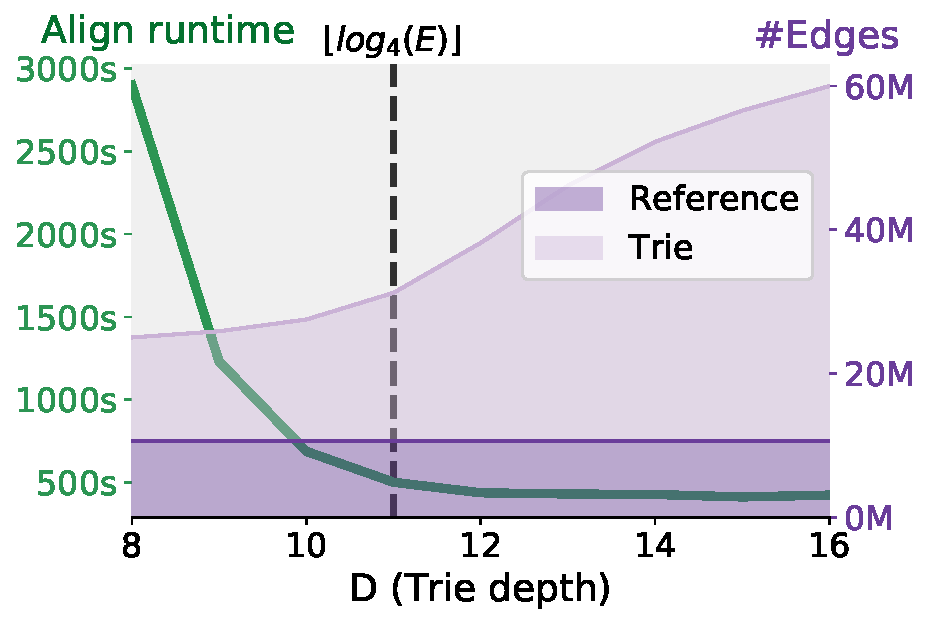
\includegraphics[width=\linewidth]{figs/trie/MHC1-trie-vs-D.pdf}
		\caption[Effect of $D$ on performance of \astarix]{Effect of $D$ on performance of \astarix (MHC1 experiment). The dashed line shows our choice of $D$.}
		%\label{subfig:MHC1-trie_vs_D}
		\label{fig:trie_vs_D}
	\end{minipage}~\hspace{0.7em}
	\begin{minipage}{0.49\linewidth}
		\centering
		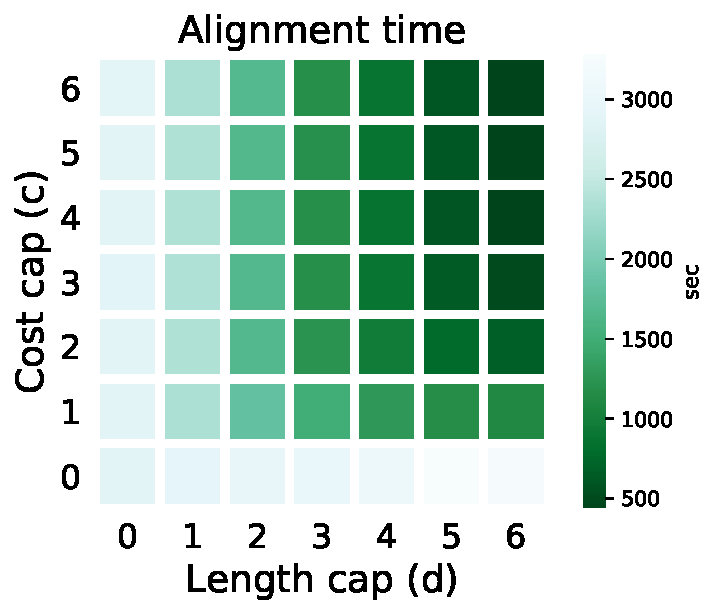
\includegraphics[width=0.8\linewidth]{figs/heuristic/MHC1-heatmap-c_vs_d-align_sec.pdf}
		\caption[Runtime of \astarix depending on $d$ and $\costcap$]{Runtime of \astarix depending on $d$ and $\costcap$ (MHC1 experiment).}
		\label{fig:heuristic-parameters}
	\end{minipage}
\end{figure}

\cref{fig:trie_vs_D} demonstrates the benefit of using a trie with the size
reduction optimization (end of \cref{subsec:trie}): increasing the trie depth
$D$ speeds up aligning but requires more memory. Selecting the trie depth based
on the graph size \mbox{$D = \lfloor \log_\Sigma \lvert \RG \rvert \rfloor$}
provides a reasonable trade-off between alignment time and memory.

\cref{fig:heuristic-parameters} shows the joint effect of $\costcap$ and $d$. It
demonstrates that having a long reach ($d$) that covers at least some errors
($\costcap > 0$) is a reasonable strategy for choosing $d$ and $\costcap$.